\paragraph{Phân tích bộ dữ liệu Credit Card Fraud} \hfill \\
Đây là bài toán cực khó với tỷ lệ dữ liệu gian lận chỉ đạt 0.172\%. Việc sử dụng Accuracy là hoàn toàn sai lầm trong ngữ cảnh này.

\paragraph{Đặc thù dữ liệu và Phân tích cấu trúc} \hfill \\
Dữ liệu đã được ẩn danh qua phép biến đổi PCA, chỉ giữ lại các cột V1-V28, cùng với thời gian (\texttt{Time}) và số tiền (\texttt{Amount}):
\begin{figure}[H]
    \centering
    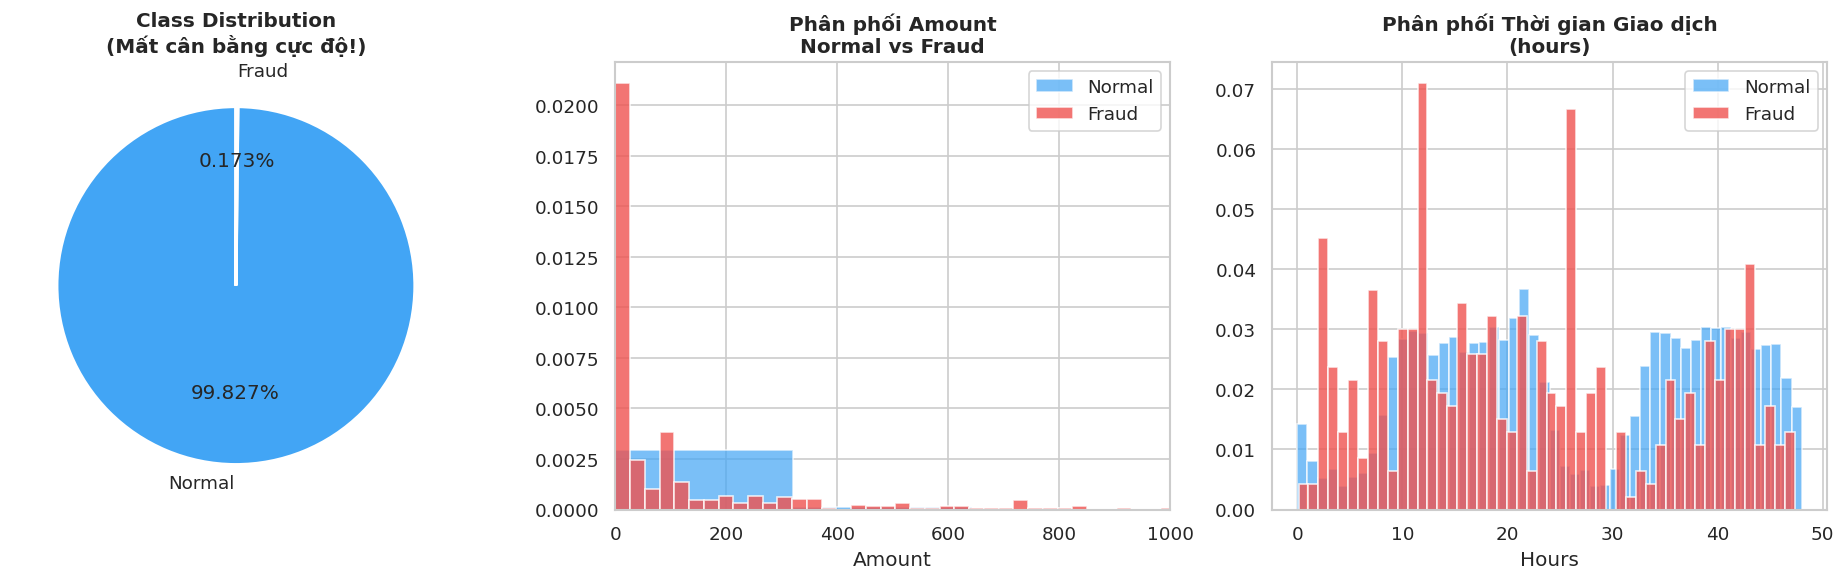
\includegraphics[width=0.8\linewidth]{Chương_1/results/credit_fraud/01_class_amount_time.png}
    \caption{Phân phối nhãn và mối liên hệ giữa Số tiền - Thời gian}
\end{figure}

Hình 1.5 cho thấy sự mất cân bằng cực độ của tập dữ liệu. Các giao dịch gian lận chiếm tỷ lệ rất nhỏ và không có sự phân hóa rõ rệt về mặt thời gian hay số tiền so với giao dịch hợp lệ, khiến việc phát hiện bằng các quy luật đơn giản là bất khả thi.

Sử dụng PCA để trực quan hóa cụm dữ liệu 2D, chúng ta thấy các vụ gian lận (màu đỏ) nằm rải rác nhưng có xu hướng tập trung ở một số vùng nhất định:
\begin{figure}[H]
    \centering
    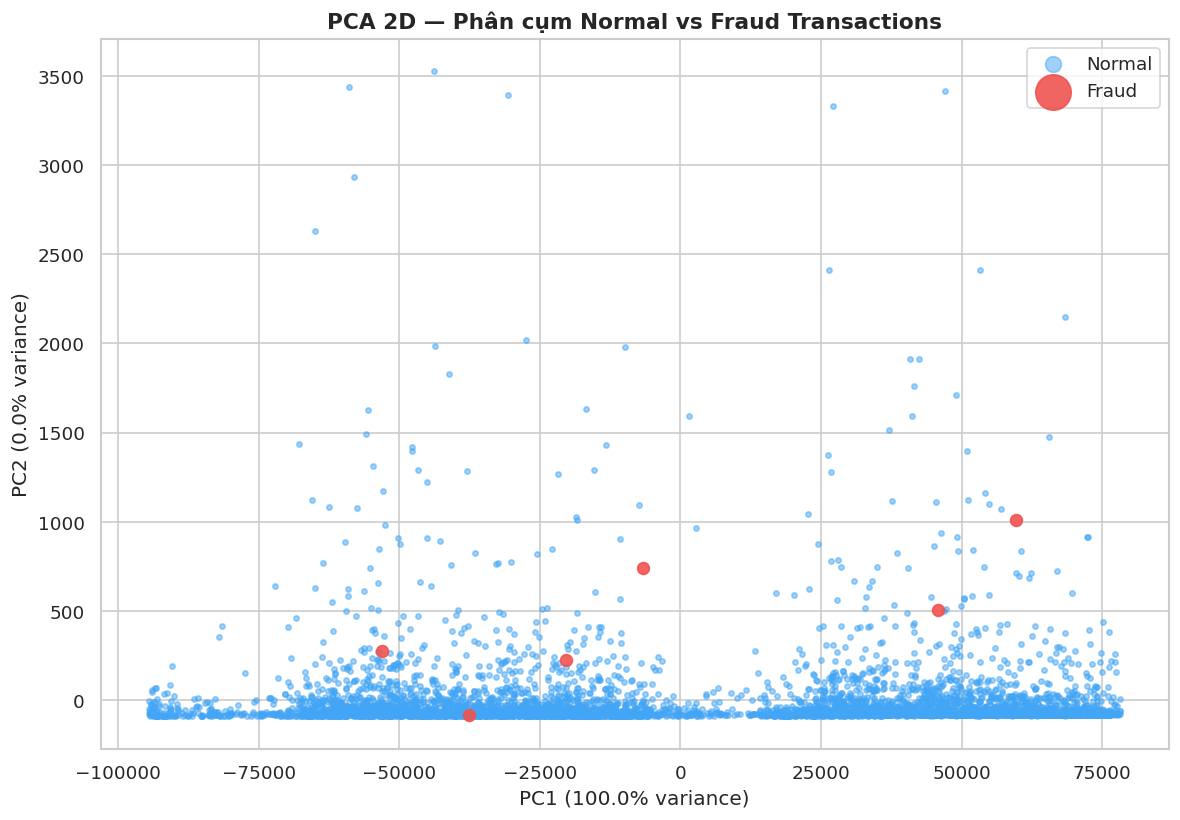
\includegraphics[width=0.8\linewidth]{Chương_1/results/credit_fraud/02_pca_2d_clusters.png}
    \caption{Trực quan hóa PCA 2D của các giao dịch}
\end{figure}

Hình 1.6 minh họa các giao dịch gian lận thông qua phép chiếu PCA xuống 2 chiều. Mặc dù có sự chồng lấn, các điểm màu đỏ (gian lận) vẫn tạo thành các cụm đặc trưng, cho phép các mô hình học máy phi tuyến tính có thể phân tách ranh giới quyết định.

Sự khác biệt về phân phối giá trị của các đặc trưng giữa giao dịch bình thường và gian lận:
\begin{figure}[H]
    \centering
    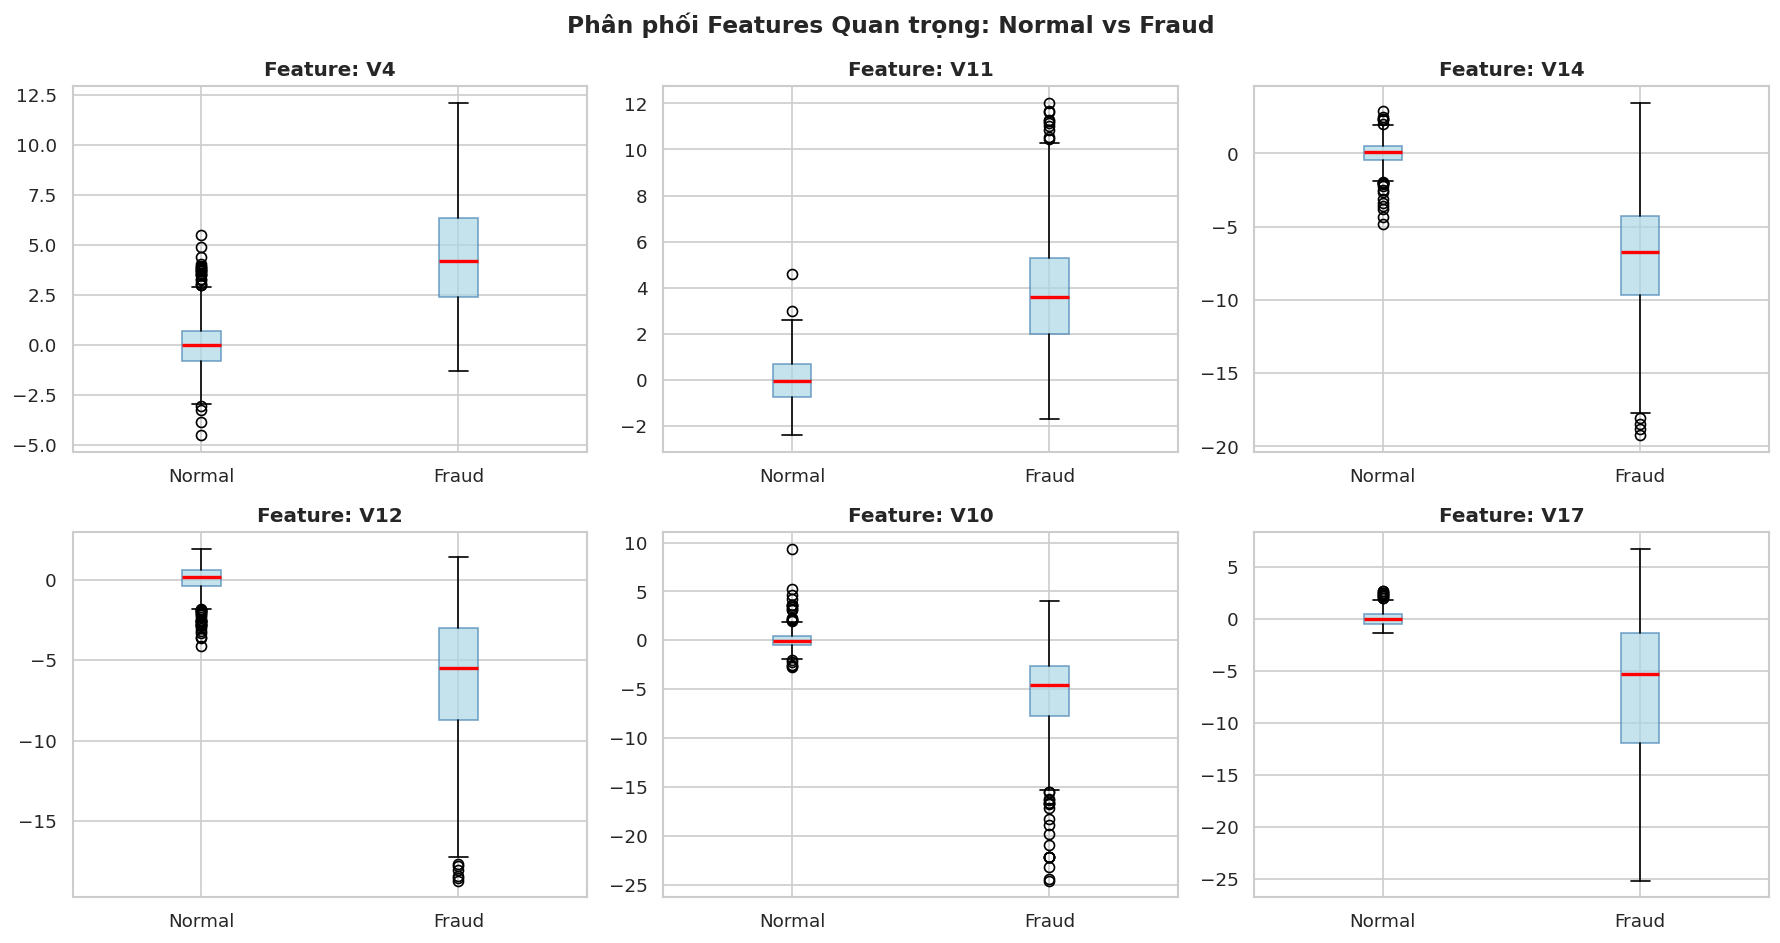
\includegraphics[width=0.8\linewidth]{Chương_1/results/credit_fraud/03_feature_boxplots.png}
    \caption{Boxplots so sánh các biến đặc trưng quan trọng}
\end{figure}

Hình 1.7 chỉ ra các biến đặc trưng có sự khác biệt lớn nhất về phân phối giữa hai lớp. Ví dụ, tại biến V14 và V17, các giao dịch gian lận thường có giá trị thấp hơn hẳn, đây là các tín hiệu quan trọng để mô hình nhận diện hành vi bất thường.

\paragraph{Kết quả thực nghiệm} \hfill \\
Chúng ta tập trung tối ưu hóa Precision-Recall (PR). Random Forest với kỹ thuật Balanced Class Weight cho kết quả rất khả thi.

\begin{table}[H]
    \centering
    \begin{tabular}{|l|c|c|c|c|}
    \hline
    \textbf{Mô hình} & \textbf{PR-AUC} & \textbf{ROC-AUC} & \textbf{Recall (Fraud)} & \textbf{Precision (Fraud)} \\ \hline
    Logistic Reg (Bal) & 0.7189 & 0.9720 & 0.92 & 0.06 \\ \hline
    \textbf{Random Forest} & \textbf{0.8653} & 0.9581 & 0.76 & \textbf{0.96} \\ \hline
    \end{tabular}
    \caption{Kết quả phát hiện gian lận (PR-AUC là chỉ số quan trọng nhất)}
\end{table}

\begin{figure}[H]
    \centering
    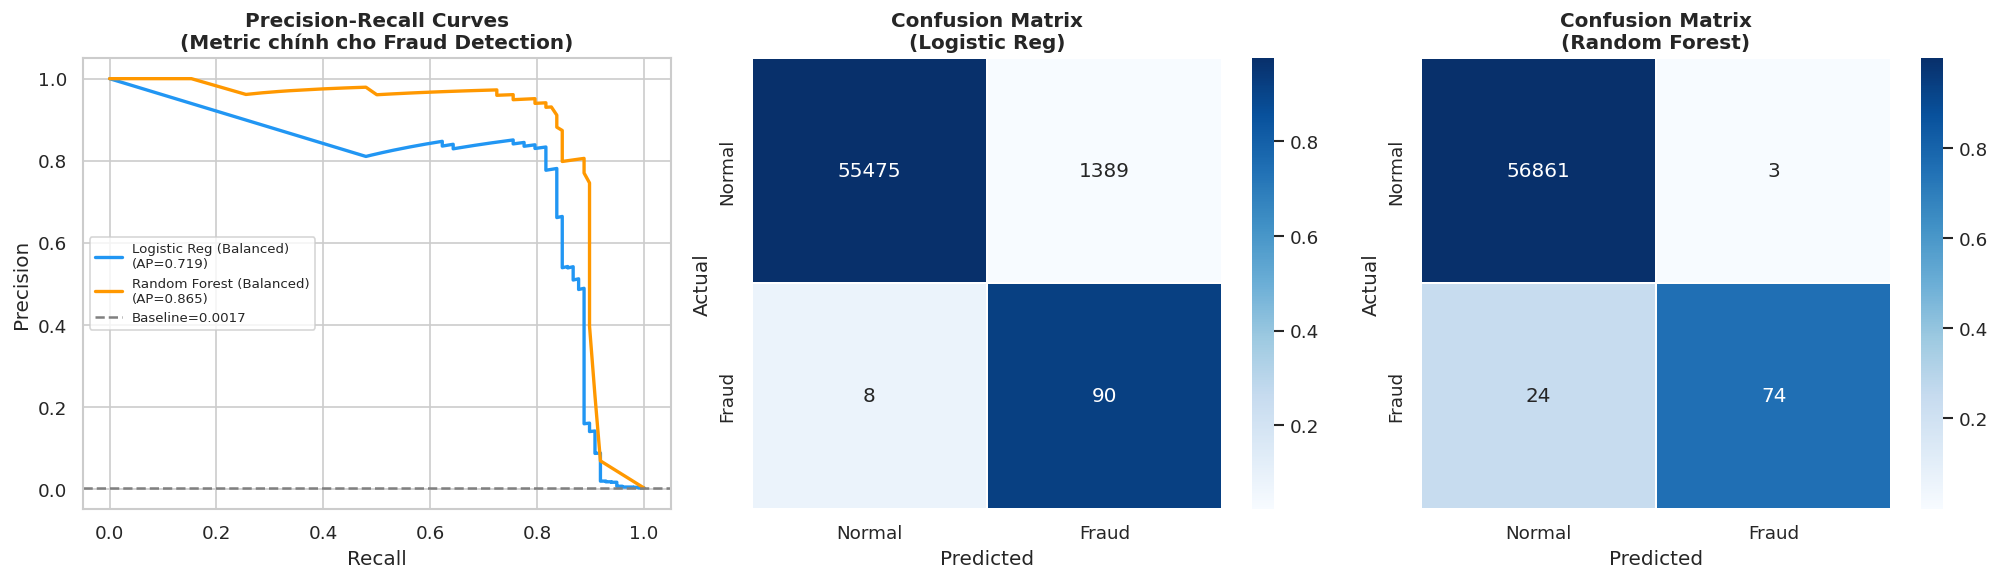
\includegraphics[width=0.8\linewidth]{Chương_1/results/credit_fraud/04_pr_curve_confusion.png}
    \caption{Đường cong Precision-Recall và Ma trận nhầm lẫn}
\end{figure}

Hình 1.8 biểu diễn đường cong Precision-Recall, một công cụ đánh giá chính xác hơn ROC trong điều kiện dữ liệu mất cân bằng. Random Forest duy trì được độ chính xác (Precision) cao ngay cả khi tăng độ bao phủ (Recall), giúp hệ thống hoạt động ổn định và tin cậy.

Random Forest đạt Precision 0.96, nghĩa là cứ 100 lần báo động gian lận thì có 96 lần là đúng, giúp giảm thiểu đáng kể chi phí kiểm tra thủ công cho ngân hàng.
    
